% Slides for 2024-07-23
% To create a slide, use the following:
\begin{frame}{Fishial}
   Testing fishial's performance on segmenting groupers 
   \centering
   \includegraphics[height=0.7\textheight,width=0.7\textwidth,keepaspectratio]{images/3_8_2024_0U1A0557_00001.png}

\end{frame}


\begin{frame}{Results}
    Having trouble picking up all the individuals
   \centering
   
\includegraphics[height=0.7\textheight,width=0.7\textwidth,keepaspectratio]{images/gm3-1.png}
   \centering
   
\includegraphics[height=0.7\textheight,width=0.7\textwidth,keepaspectratio]{images/gm3-2.png}

\end{frame}


\begin{frame}{Segmenting with bounding boxes}
    Segmented the groupers that are close to the camera
    \centering
   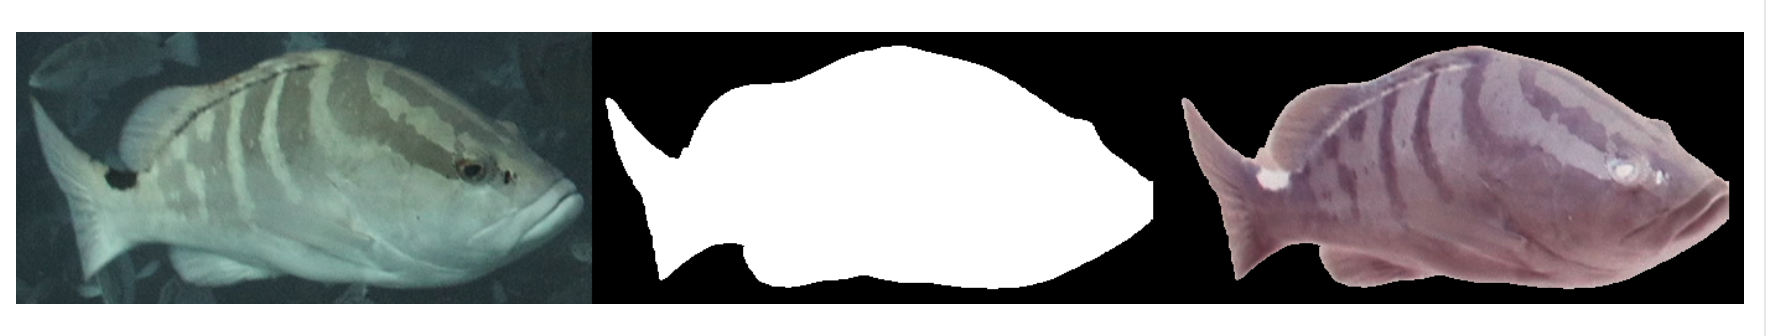
\includegraphics[height=0.7\textheight,width=0.7\textwidth,keepaspectratio]{images/gm3-3.png}
   \centering
   
\includegraphics[height=0.7\textheight,width=0.7\textwidth,keepaspectratio]{images/gm3-4.png}
   \centering
   
\includegraphics[height=0.7\textheight,width=0.7\textwidth,keepaspectratio]{images/gm3-5.png}
   

\end{frame}

\begin{frame}{Segmenting with bounding boxes}
    It was not able to pick up the groupers in the background 
    \centering
   
\includegraphics[height=0.7\textheight,width=0.7\textwidth,keepaspectratio]{images/gm3-6.png}
   \centering
   
\includegraphics[height=0.7\textheight,width=0.7\textwidth,keepaspectratio]{images/gm3-7.png}
   
\end{frame}


% To create a slide with a bullet list, use the following:
% \begin{frame}{TITLE}
%     \begin{itemize}
%         \item ITEM 1
%         \item ITEM 2
%     \end{itemize}    
% \end{frame}

% To create a slide with numbered list, use the following:
% \begin{frame}{TITLE}
%     \begin{enumerate}
%         \item ITEM 1
%         \item ITEM 2
%     \end{enumerate}
% \end{frame}

% To create a slide with a graphic:
% 1. Add the graphic to this folder (named picture.png)
% 2. Use the following:
% \begin{frame}{TITLE}
%     \centering
%     \includegraphics[height=0.7\textheight,width=0.7\textwidth,keepaspectratio]{picture.png}
% \end{frame}

% To create a slide with two columns, use the following:
% \begin{frame}{TITLE}
%     \begin{columns}
%         \begin{column}{0.5\textwidth}
%             COLUMN 1 BODY
%         \end{column}
%         \begin{column}{0.5\textwidth}
%             COLUMN 2 BODY
%         \end{column}
%     \end{columns}
% \end{frame}
